\chapter{On control of harmonic waves in  an acoustic metamaterial}

Generation of harmonic waves in a mass-in mass model of an acoustic metamaterial is considered. It is shown numerically that outside the band gap, the boundary harmonic excitation gives rise to a formation of periodic waves whose profile gradually coincides with the profile of the exact travelling wave harmonic solution. No waves are generated by the boundary excitation inside the band gap. A switch-on/off control is developed to achieve the formation of the harmonic waves inside the band gap.
  
\section{Introduction}

The interest to the study of the acoustic metamaterials has grown considerably in the recent years, see \cite{Cummer,Cvet, Huang2010, Ma, muller, delis1, Eremeyev2020, Porubov2019, Erofeev2020} and references therein. The linear acoustic metamaterials draw  more attention \cite{Cvet, Huang2010,  muller}. One of the simplest but instructive model is the mas-in-mass model. It allows to describe the band gap in the dispersion relation \cite{Cvet, Huang2010}, negative effective mass  and other features related to a metamaterial. 

Experimental realization of the mass-in-mass  model may be found in \cite{Cvet,Yang, Yao2008, Zhou2015}. The existence of band gap was confirmed there. However, no periodic waves were recorded. The metamaterial has been constructed in \cite{Yang} so as to change the internal oscillator by an electric signal. Similarly the 
 external electromagnetic signals were used in \cite{Chen2014,Xiao2015} to develop the active tunable acoustic metamaterials. One can note the luck of theoretical results concerning generation of the harmonic waves and their control.

In this paper we study numerically generation  of harmonic waves in  a linear metamaterial mass-in-mass model.  The boundary harmonic excitation is shown to produce both the acoustic and optic harmonic waves outside the band gap while no wave propagation is obtained inside the bamd gap. Then the switch-on/off control is developed to see how to change the shape of the harmonic waves inside and outside the band gap.

\section{Statement of  problem}

Consider a  chain   when interaction between the  masses,  $m$,  is modeled by linearly- elastic springs \cite{Huang2010}. An elastic internal oscillator is modelled by the additional masses $m_1$ , attached by springs to each mass $m$ in the chain, and this interaction is also linear and elastic. Masses $m_1$ do not interact directly between themselves. The displacement of the mass $m$ with the number $n$ is denoted by $x_n$, while that of $m_1$ is denoted by $y_n$.

\begin{equation}
\ddot{x_n}=\beta_0 (x_{n-1}-2x_n+x_{n+1})+\eta \beta_1 (y_n-x_n), 
\label{eq1}
\end{equation}
\begin{equation}
\ddot{y_n}=-\beta_1 (y_n-x_n). \label{eq2}
\end{equation}
Here $\eta=m_1/m$, while the linear stiffness of the spring of the chain is $\beta_0 m$,  the nonlinear stiffness is $\beta_3 m$. Corresponding linear and nonlinear stiffnesses of the attached spring are $\beta_1 m_1$ , $\beta_2 m_1$ respectively. 
\begin{figure*}[h]
\begin{center}
%\begin{flushleft}
%\end{flushleft}
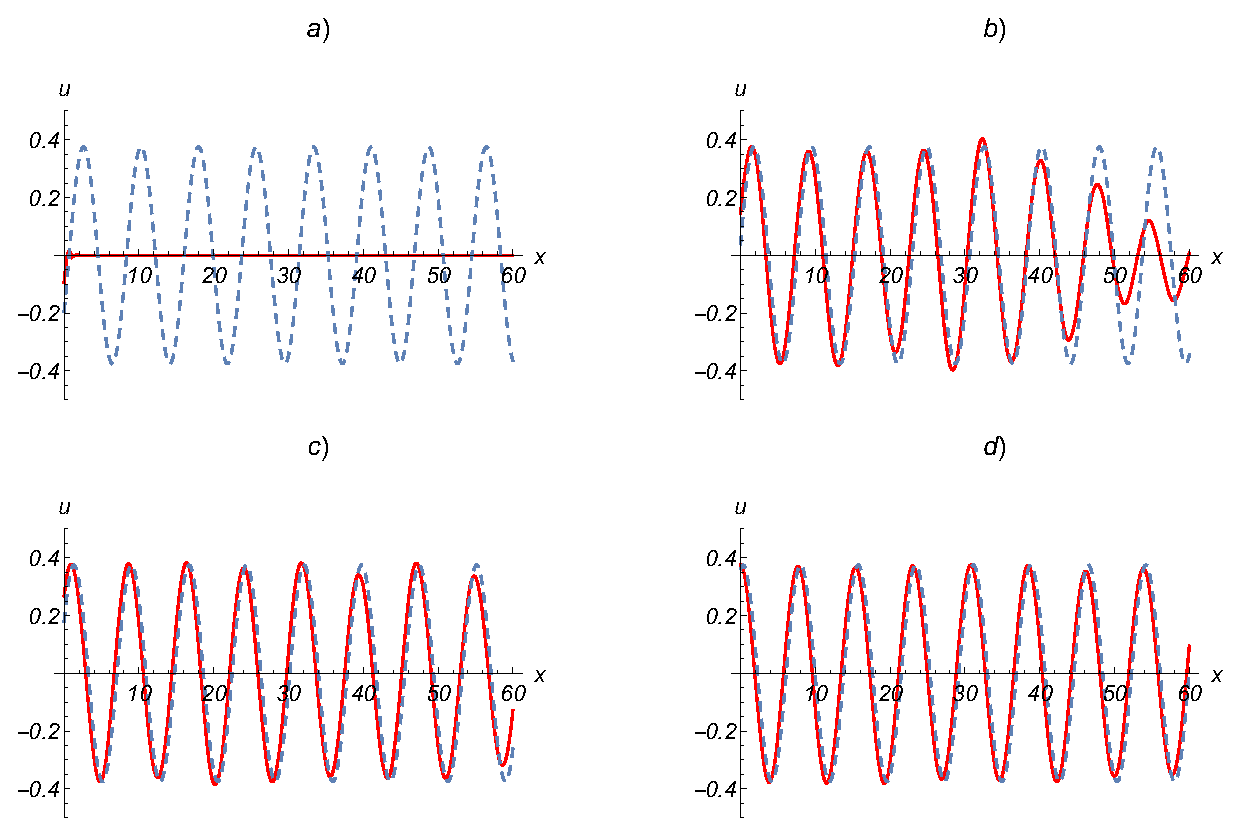
\includegraphics[width=1.0\textwidth]{new_pic/fig1.eps}
\end{center}
\caption{ Evolution of $u$ wave below the band gap, $\omega<\sqrt{\beta_1}$. Shown by dashed line is the imagine part of the  exact solution (\ref{solfin}) with the frequency $\omega=\omega_a$.  a)$t=0$; b)$ t=t_N/4$; c) $t=t_N/2$, d)$t=t_N$.}
\label{fg1}
  \end{figure*}
We proceed with a continuum limit of Eqs. (\ref{eq1}), (\ref{eq2}). Following the standard procedure we introduce the continuum functions $u(x,t)$, $v(x,t)$ for description of the displacements of the masses $m$, $m_1$ with the number $n$ while the continuum displacements of the neighboring masses are sought using the Taylor series around $u$. Retaining only the first nonzero term in the expansion we obtain
\begin{equation}
u_{tt}=\beta_0 h^2 u_{xx}+\eta \beta_1 (v-u), \label{eq3}
\end{equation}
\begin{equation}
v_{tt}=-\beta_1 (v-u), \label{eq4}
\end{equation}
where $h$ is a distance between the masses $m$ in the chain. 
The conventional traveling wave solution is sought as 
\begin{equation}\label{sol}
 u=A\exp (\imath(p~ x - \omega~ t- p~ x_0)), ~
   v=B \exp (\imath(p~ x - \omega~ t-p~ x_0))
\end{equation}
Substituting Eq. (\ref{sol}) into Eqs. (\ref{eq3}), (\ref{eq4}) one obtains the known dispersion relation \cite{Huang2010} 
\[
\omega^4 -(\beta_1(1+\eta)+\beta_0 p^2 h^2)\omega^2+\beta_0 \beta_1 p^2 h^2=0.
\]
whose solution is 
\begin{equation}\label{acdiscr}
\omega_a^2=\frac{\beta_1(1+\eta)+\beta_0 h^2 p^2}{2}-\frac{\sqrt{D}}{2},
\end{equation}
\begin{equation}\label{optdiscr}
\omega_o^2=\frac{\beta_1(1+\eta)+\beta_0 h^2 p^2}{2}+\frac{\sqrt{D}}{2},
\end{equation}
where
\[
D=(\beta_1(1+\eta)+\beta_0 h^2 p^2)^2-4\beta_0 h^2 p^2,
\]

Also the expression for $A$ through  $B$ is obtained giving rise to the solution for $u$ and $v$ in the final form
\begin{equation}\label{solfin}
 u=\frac{\beta_1-\omega^2}{\beta_1}~B\exp (\imath(p~ x - \omega~ t- p~ x_0)), ~
   v=B \exp (\imath(p~ x - \omega~ t- p~ x_0)),
\end{equation}
where the frequency is  $\omega=\omega_a$,  or $\omega=\omega_o$, $x_0$ accounts for an initial phase.
The acoustic band frequency varies from $0$ to $\sqrt{\beta_1}$\, while the optic one lies in the interval 
$(\sqrt{\beta_1(1+\eta)}, \infty)$. Therefore, there is a band gap $\sqrt{\beta_1}<\omega<\sqrt{\beta_1(1+\eta)}$ where no harmonic traveling wave propagates.

\section{Generation of harmonic waves}
The analysis in the previous Section is based on the particular traveling wave solution which requires specific initial and boundary conditions for its realization. However, experimental generation of the waves in a metamaterial uses the boundary excitation of the waves. In particular, the following  initial and boundary conditions for $u$ can be employed,
\begin{equation}\label{bcu}
u(0,t)=\frac{\beta_1-\omega^2}{\beta_1}~B~ {\text{sin}} (\omega ~t),~u(x,0)=0, ~u(x,0)_t=0,
\end{equation}
while for $v$ we assume that
\begin{equation}\label{bcv}
v(0,t)=B ~{\text{sin}} (\omega ~t),~v(x,0)=0, ~v(x,0)_t=0,
\end{equation}
This problem can be solved numerically. The Wolfram Mathematica NDSolve command is used to solve Eqs. (\ref{eq3}), (\ref{eq4} with the conditions (\ref{bcu}), (\ref{bcv}). 
%The interval of calculations is $0<x<x_N$,
The interval of interest is $0<x<x_N$, 
 the absorbing boundary conditions %for $u$, $v$ 
are imposed at $x=x_N$%.
 using the following masking technique. The calculation domain $0 < x < 3 x_N$ is being splitted into two parts:  $0 < x < x_N$ and  $x_N < x < 3 x_N$ while the system of Eq.  (\ref{eq1}), (\ref{eq2}) is replaced with
$$
U_{t}=\beta_0 h^2 u_{xx}+\eta \beta_1 (v-u)
$$
$$
u_{t}=U + u f_{\text{mask}},
$$
$$
v_{tt}=-\beta_1 (v-u),
$$
where $f_{\text{mask}} = \log \left(\tanh{0.03 (3 x_N - x)}\right)^2$. By this way, as far as $f_{\text{mask}}$ is effectievely zero in the interval of interest the exact system of Eq.  (\ref{eq1}), (\ref{eq2}) is being solved there. While for the rest part of the domain $f_{\text{mask}}$ is negative and decreasing with $x$,4 which leads to the corresponding decrease of the amplitude of the each wave frequency traveling through. The resulting amplitude of wave at $x = 3 x_N$ becames numerically very close to zero leading to nothing be reflected to the interval of interest from the $x = 3 x_N$ boundary.
\begin{figure*}
\begin{center}
%\begin{flushleft}
%\end{flushleft}
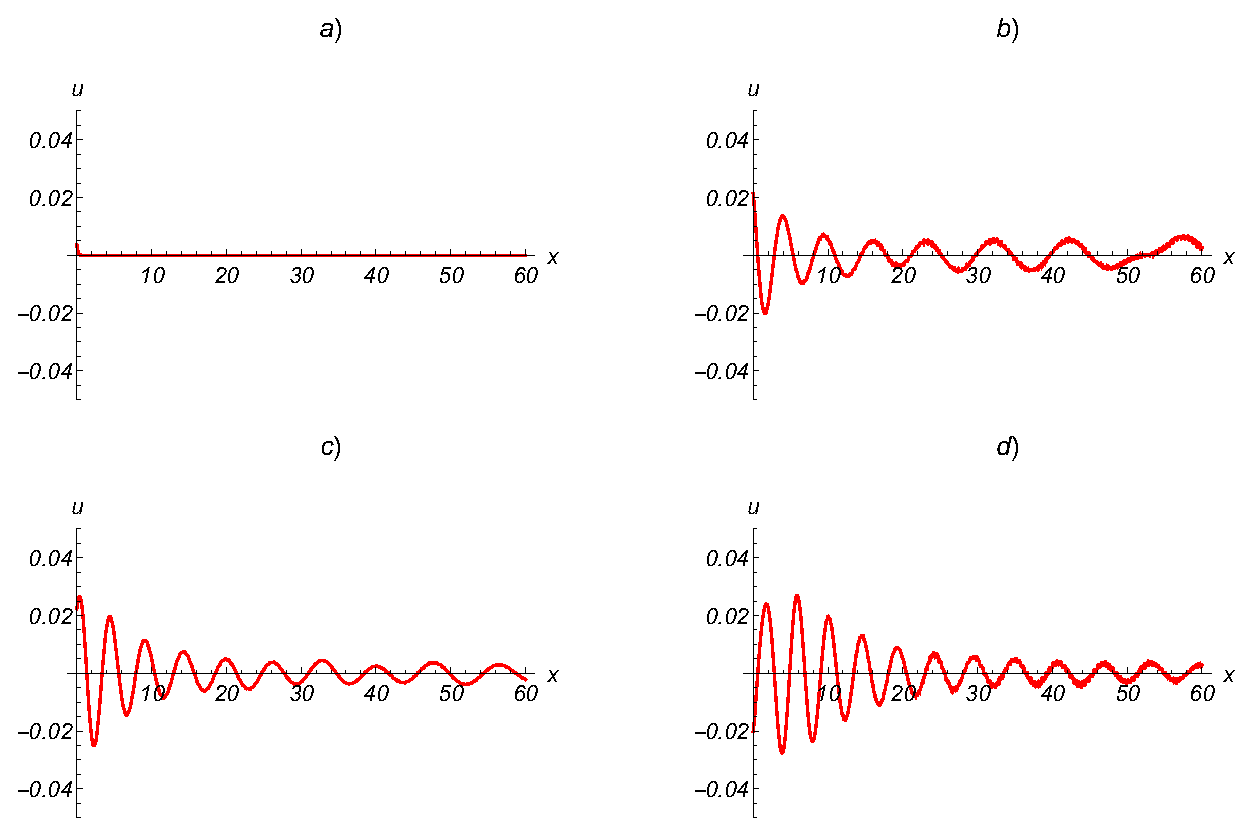
\includegraphics[width=1.0\textwidth]{new_pic/fig2.eps}
\end{center}
\caption{ Evolution of $u$ wave at the lower boundary of the band gap, $\omega \approx \sqrt{\beta_1}$,  $\omega=0.3$.  a)$t=0$; b)$ t=t_N/4$; c) $t=t_N/2$, d)$t=t_N$.}
\label{fg2}
  \end{figure*}



  
The aim of calculations is to see how the harmonic boundary excitation gives rise to the harmonic wave  in time.  The imaginary parts of the solutions (\ref{solfin}) will be compared with the numerical results. For this purpose the initial position $x_0$  in Eqs. (\ref{solfin}) will be chosen so as to coincide as close as possible the numerical and analytical curves at the final time of calculations, $t=t_N$. Then both curves are placed together for the preceding moments of times. Also, the realization of the band gap will be studied by varying the frequency $\omega$ ib the boundary conditions (\ref{bcu}), (\ref{bcv}) from zero through the band gap. Therefore the values of frequency $\omega$ is defined while the wave number of the exact solution, $p$, is calculated through it using the dispersion relation,
\[
p=\omega\sqrt{\frac{\beta_1(1+\eta)-\omega^2}{\beta_0 h^2(\beta_1-\omega^2)}}.
\]
The values of the coefficients are chosen as 
$t_N = 600; x_N = 60;\beta_0=1, h = 0.5; \beta_1 = 0.1; \eta = 0.5;  B=0.25$. Then the band gap is $0.316<\omega<0.387$.

  
Shown in Fig \ref{fg1} is the formation of harmonic wave $u$ at various times when the excitation frequency lies below the band gap, $\omega<\sqrt{\beta_1}$, $\omega=0.2$, $x_0= 15.8$. The exact solution is placed on each time sketch a)-d).  One can see that initially undisturbed stage a) transforms to a non-harmonic wave which partially coincides with the harmonic exact traveling wave solution at the stage b). The last two stages c) and d) demonstrate almost full similarity between numerical and analytical solution.
\begin{figure*}
\begin{center}
%\begin{flushleft}
%\end{flushleft}
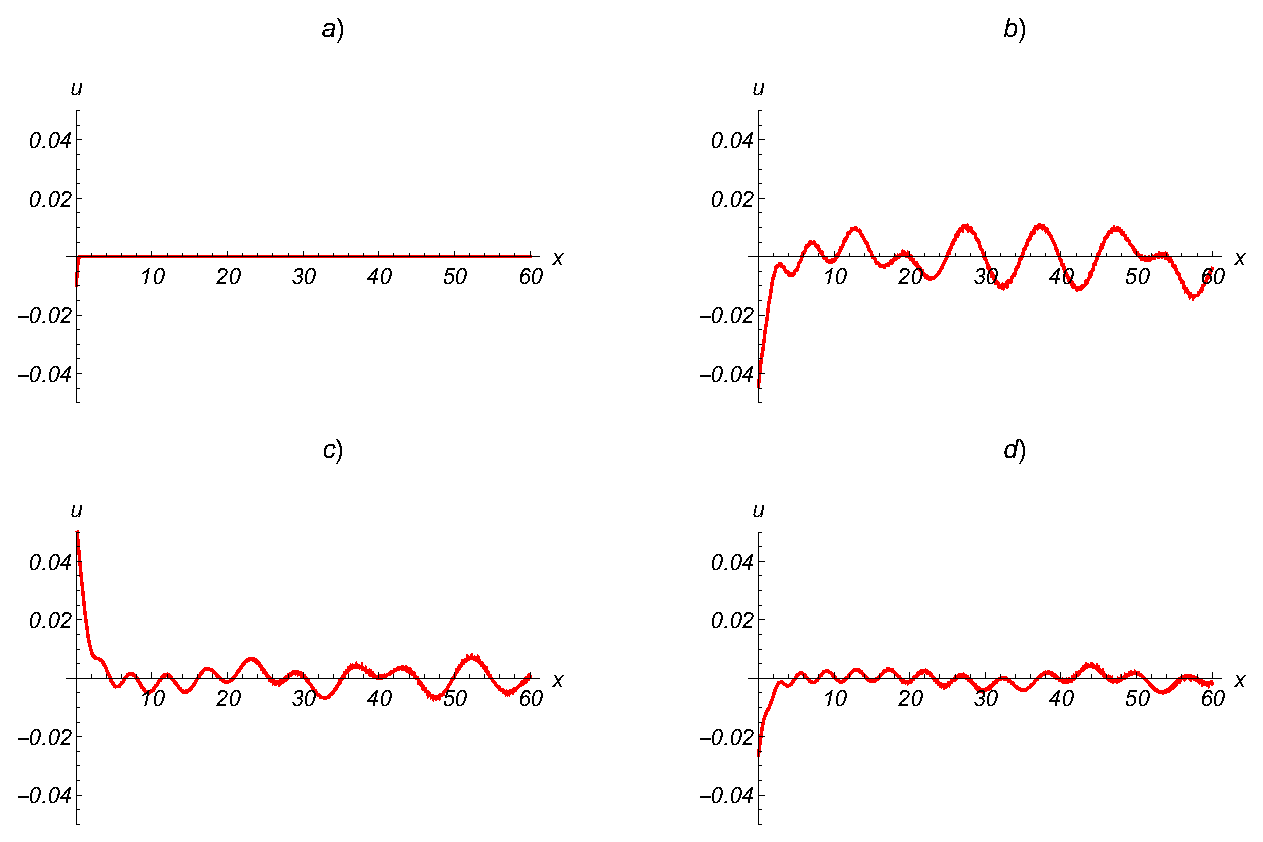
\includegraphics[width=1.0\textwidth]{new_pic/fig3.eps}
\end{center}
\caption{Supression  of $u$ wave inside the band gap, $\sqrt{\beta_1}<\omega<\sqrt{\beta_1(1+\eta)}$, $\omega=0.35$. a)$t=0$; b)$ t=t_N/4$; c) $t=t_N/2$, d)$t=t_N$.}
\label{fg3}
  \end{figure*}
  
An increase in the excitation frequency up to  the lower boundary of the band gap, $\omega \approx \sqrt{\beta_1}$,  $\omega=0.3$,  results in the formation of the wave shown in Fig. \ref{fg2}. One can see no harmonic wave generation, the amplitude of the wave decays away from the left boundary. The last two stages c) and d) demonstrate almost stable wave dynamics.
\begin{figure*}
\begin{center}
%\begin{flushleft}
%\end{flushleft}
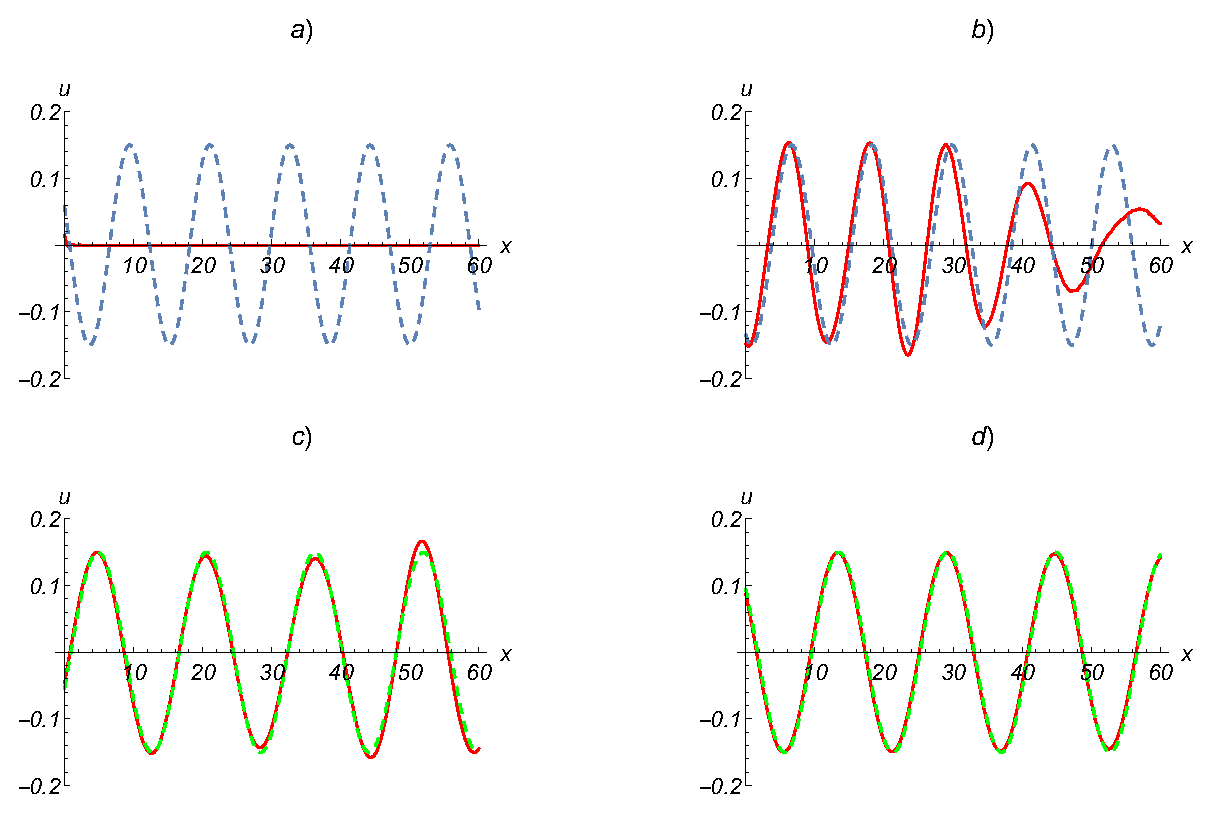
\includegraphics[width=1.0\textwidth]{new_pic/fig4.eps}
\end{center}
\caption{ Control of evolution of $u$ wave below the band gap, $\omega<\sqrt{\beta_1}$ when the control switches-on at $t=t_N/4$.   a)$t=0$; b)$ t=t_N/4$. Shown by dashed line is the imagine part of the  exact solution (\ref{solfin}) ; c) $t=t_N/2$, d)$t=t_N$. Shown by dashed line is the imagine part of the  exact solution (\ref{solwave}) }
\label{fg4}
  \end{figure*}
\begin{figure*}
\begin{center}
%\begin{flushleft}
%\end{flushleft}
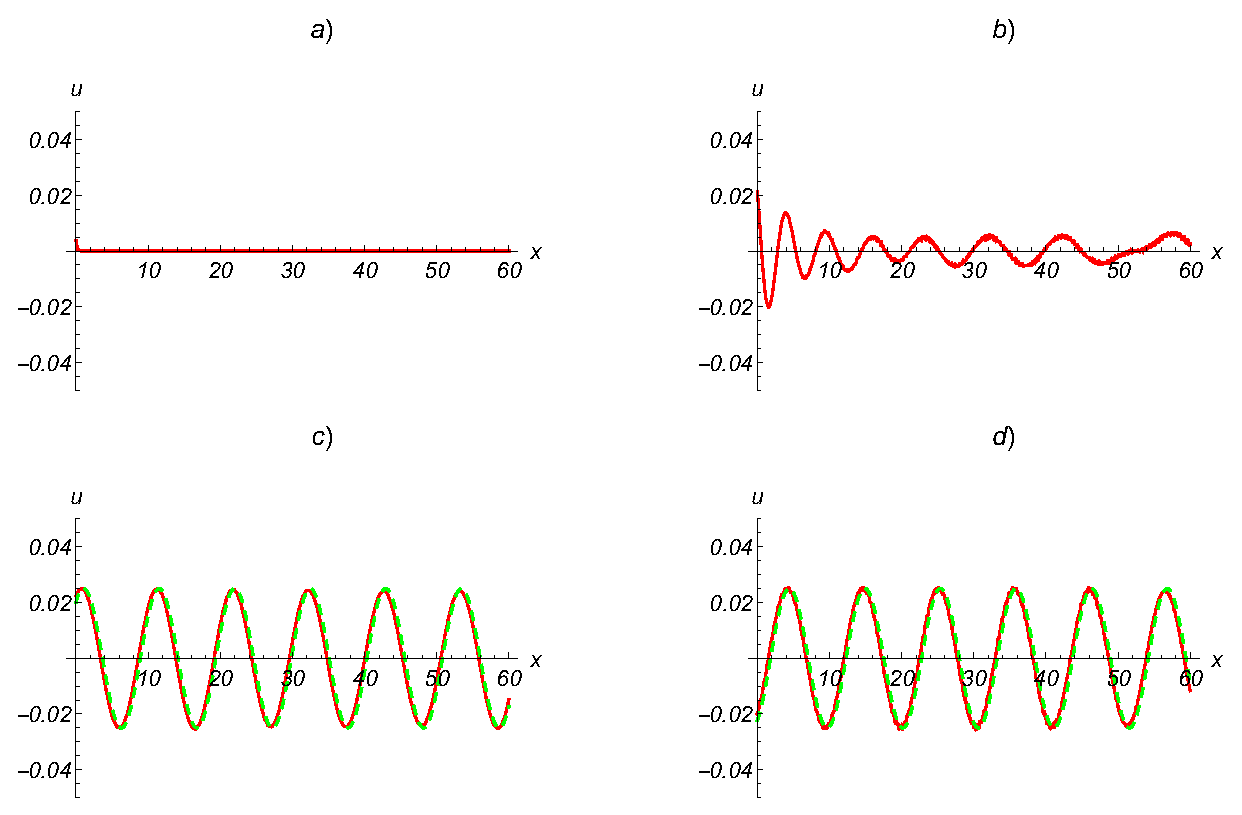
\includegraphics[width=1.0\textwidth]{new_pic/fig5.eps}
\end{center}
\caption{Control of evolution of $u$ wave at the lower boundary of  the band gap, $\omega \approx \sqrt{\beta_1}$, $\omega=0.3$,  when the control switches-on at $t=t_N/4$.   a)$t=0$; b)$ t=t_N/4$ ; c) $t=t_N/2$; d)$t=t_N$. Shown by dashed line in the last two stages  is the imagine part of the  exact solution (\ref{solwave}) .}
\label{fg5}
  \end{figure*}
  
  \begin{figure*}[ht]
\begin{center}
%\begin{flushleft}
%\end{flushleft}
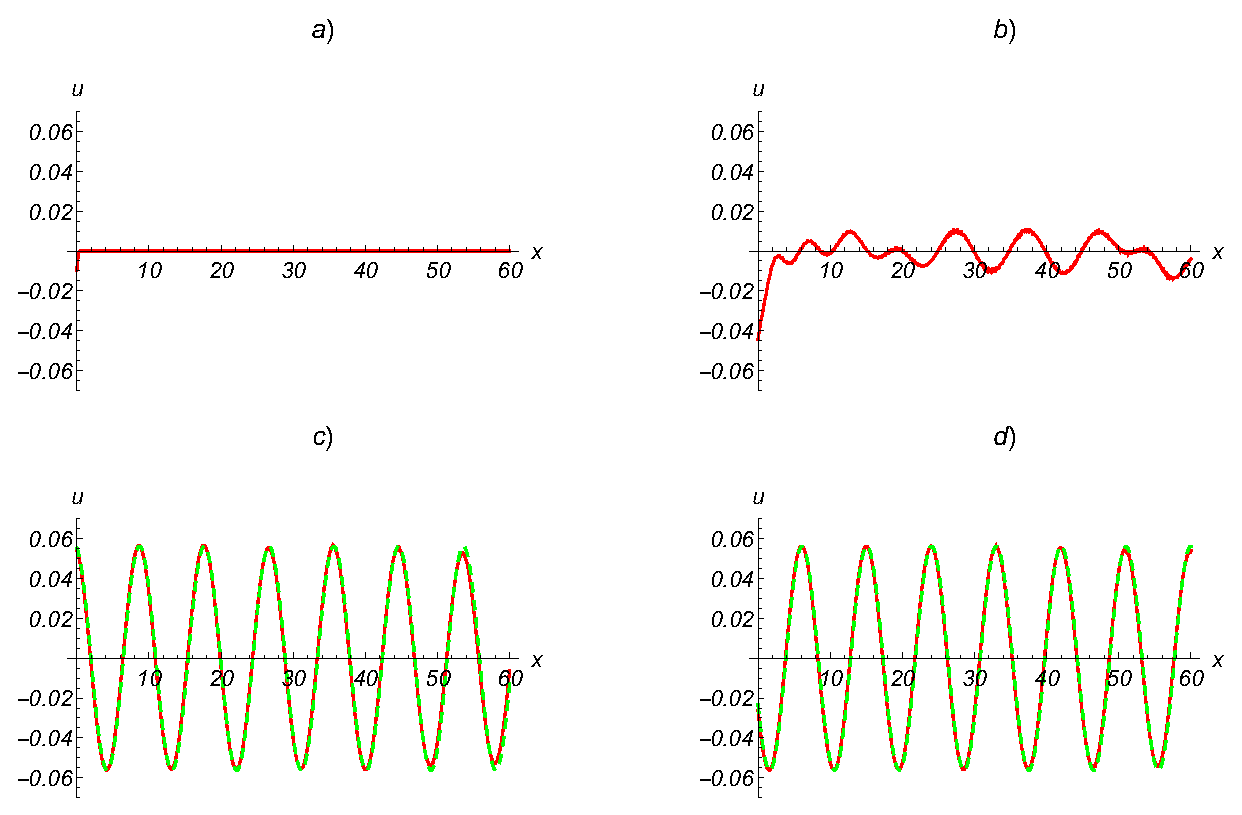
\includegraphics[width=1.0\textwidth]{new_pic/fig6.eps}
\end{center}
\caption{Control of evolution of $u$ wave inside  the band gap, $\omega=0.35$,  when the control switches-on at $t=t_N/4$.   a)$t=0$; b)$ t=t_N/4$ ; c) $t=t_N/2$; d)$t=t_N$. Shown by dashed line in the last two stages  is the imagine part of the  exact solution (\ref{solwave}) .}
\label{fg6}
  \end{figure*}
Inside the band gap, $\sqrt{\beta_1}<\omega<\sqrt{\beta_1(1+\eta)}$,  $\omega=0.35$ there is no even a wave with decreasing amplitude. Shown in Fig.\ref{fg3} is a stromg decrease in the amplitude of disturbances and their chaotic character. This is in an agreement with the analysis from the previous Section.



Further increase in the value of the excitation frequency results in the realization of the dynamics shown in Fig. \ref{fg2} when the frequency achieves the value of the upper boundary of band gap. At higher frequencies a formation of periodic wave happens with the frequency belonging to the optic branch, $\omega=\omega_o$. Again the similarity with the exact solution is observed like that shown in Fig.\ref{fg1}.


  
\section{Control of harmonic waves}

The use of electromegnetic signals  in \cite{Yang,Chen2014,Xiao2015} to change the internal properties of a metamaterial suggests the mechanism of a control based on an instant switch-on. It is modelled by the unit step function $H(t_0-t)$ that switches-off  the coupling in Eqs.  (\ref{eq3}), (\ref{eq4}) at$t=t_0$. Thus, for $u$ we have

\[
u_{tt}=\beta_0 h^2 u_{xx}+\eta \beta_1 (v-u)~H(t_0-t)
\]
Also, the unit step function should be added in equation of motion  (\ref{eq4}) and  boundary condition for $v$ (\ref{bcv}). The switch-on time for the control , $t_0$, is chosen equal to $t_N/4$, other parameters of calculations are the same as in the previous Section.

Again the comparison with the exact solution will be given.  However, after switch-on the control, equation of motion for $u$ becomes the linear wave equation whose solution is 
\begin{equation}\label{solwave}
 u_w=\frac{\beta_1-\omega^2}{\beta_1}~B~{\text{sin}}  (\imath(\omega/a~ x - \omega~ t-\omega/a~ x_0))
 \end{equation}
 Then the comparison will be done with different solutions before and after switch-on the control.
 
 Shown in Fig \ref{fg4} is the generation of the harmonic waves at $\omega=0,2$ when the control switches on at the stage b).  A comparison with the solution (\ref{solfin}) demonstrates partial similarity between the analytical and numerical solution. However, contrary to Fig. \ref{fg1}, the stages c) and d) show the tendency to the solution (\ref{solwave}) . So the control provides a transition from one harmonic wave to another.

An increase in the excitation frequency up to the lower boundary of the band gap shown in Fig. \ref{fg5} did not result in the harmonic wave without control as shown in Fig. \ref{fg2}. Here the switch-on the control at 
$t_0=t_N/4$ results in the formation of the harmonic wave whose shape is close to the analytical solution shown by dashed line  (\ref{solfin}) .

The same happens for the excitation frequency $\omega=0.35$ inside the band gap. Shown in Fig. \ref{fg6} is the formation of the harmonic wave whose shape is close to the analytical solution shown by dashed line  (\ref{solfin})  contrary to the no propagation scenario shown in Fig. \ref{fg3}.



\section{Discussion}

The boundary excitation can generate harmonic waves in the metamaterial in an agreement with the results obtained on the basis of the particular traveling wave solution. However, the area of the values of the frequency where no periodic waves propagates turns out wider than that predicted by the analysis of the dispersion relation. Besides the band gap zone where no waves propagate, there is an interval where non-periodic waves travel.

The switch-on control allow us to provide harmonic waves generation inside and outside the band gap. Such mechanism of control could be realized using the experimental set-up developed in \cite{Yang}. Similar to this paper, one can not only switch- off the internal oscillator but change its properties.

Further perspectives could be related to the active metamaterial with an external force accounting for the feedback control \cite{Pope2012,Pope2014}. In this case application of the feedback speed-gradient control  method developed in our early works \cite{Fradkov2007,  Porubov etal.2016}, looks promising. Of special interest is the inclusion of nonlinearity in the model of the metamaterial and development of the nonlinear methods of control.